\documentclass[11pt]{article}
\usepackage[margin=1in]{geometry}
\usepackage{amsmath,amssymb,booktabs,array,longtable,tabularx,graphicx,xcolor}
\usepackage{tikz}
\usetikzlibrary{arrows.meta,positioning,fit,shapes.geometric}
\usepackage{hyperref}
\usepackage[numbers,sort&compress]{natbib}
\setlength{\parindent}{0pt}
\setlength{\parskip}{0.65\baselineskip}
\newcommand{\ccmname}{Cortical-Column Memory (CCM)}
\newcommand{\releaseversion}{v0.1.0}
\newcommand{\statusline}{Architecture and Preregistered Evaluation Protocol}
\hypersetup{colorlinks=true,linkcolor=blue,citecolor=blue,urlcolor=blue,pdftitle={Cortical-Column Memory}}

\title{Cortical-Column Memory: A Thousand-Brains-Inspired Memory and Consensus Architecture for Resource-Constrained Multi-Agent Systems\\[0.4em]
\large System Design, Implementation, and Preregistered Evaluation Protocol}
\author{James Booth\\Independent researcher\\\url{https://github.com/jmsbooth/agentic-cortical-column-memory}}
\date{September 3, 2026\\\small \releaseversion{} · \statusline{} · Preprint, not peer reviewed}

\begin{document}
\maketitle

\begin{abstract}
Resource-constrained deployments cannot always purchase larger models, longer context, or unconstrained inference. This paper proposes \ccmname{}, an engineering architecture that tests whether modular state surrounding a small model can recover selected capabilities associated with model scale. CCM translates four ideas associated with the Thousand Brains literature into explicit software contracts: navigable reference frames, local column models, provenance-bearing structured memory, and active evidence gathering coordinated by structured hypothesis consensus. The translation is an architectural hypothesis, not a claim of biological realism or cortical equivalence. This \releaseversion{} release publishes the reference implementation, deterministic synthetic task environments, baselines, component ablations, resource accounting, statistical decision rules, and machine-readable run manifests before the registered empirical campaign is completed. It therefore exposes a falsifiable validation framework rather than reporting a completed empirical study. The registered questions distinguish architectural benefit from additional test-time computation and retain abstention, unresolved disagreement, and negative findings as valid outcomes.
\end{abstract}

\textbf{Publication state.} The registered experimental campaign has not been completed. This release publishes the architecture, implementation, hypotheses, baselines, metrics, and decision criteria before final data collection. The only executable measurements included at release time are software smoke-test artifacts, clearly labelled as such in the repository.

\section{Introduction}

AI agents operate across observations, actions, and changing world state. Their current prompt is not persistent memory: a long transcript may contain irrelevant material, a summary may erase the source of a claim, similarity retrieval may mix incompatible times, and a flat episodic record may not expose relations or supersession. These failures can force a reasoning model to repeatedly reconstruct state that an agent could instead maintain explicitly.

This paper asks whether persistent agent memory should be organized primarily as multiple bounded structured models of an observed world rather than as retained text or retrieval over historical text. The proposed answer is Cortical-Column Memory (CCM), a model-agnostic memory architecture in which local modeling units maintain observations relative to reference frames, preserve temporal history and provenance, derive state and hypotheses, and reconcile partial representations into bounded recall context.

\subsection{The architectural question}

The central question is:

\begin{quote}
Does structured modular world-state memory improve relevant recall, temporal consistency, relational reconstruction, provenance, and downstream agent performance compared with conventional memory architectures under matched task and resource conditions?
\end{quote}

The Thousand Brains literature motivates the design vocabulary of local models, reference-frame-relative structure, partial representations, and active interaction \citep{hawkins2017columns,hawkins2019framework}. CCM makes an engineering interpretation of selected principles. It does not claim that a software column is a cortical column, that the implementation reproduces neuroscience, or that TBT is necessary for the architecture to be useful.

\subsection{Contributions and boundaries}

The contributions of this release are:

\begin{enumerate}
  \item a memory-first CCM architecture in which an agent may contain multiple bounded columns;
  \item explicit contracts for observations, relations, state, hypotheses, transitions, predictions, reference frames, temporal validity, recall, context assembly, and reconciliation;
  \item a dependency-free reference implementation with a deterministic symbolic adapter and a provider-neutral model adapter interface;
  \item a preregistered evaluation matrix centered on conventional memory baselines, memory-specific tasks, memory-quality metrics, resource costs, and component ablations; and
  \item a reproducible validation harness that emits provenance-bearing traces and machine-readable manifests without fabricated campaign results.
\end{enumerate}

Small-model efficiency and multi-agent composition remain useful secondary questions. A multi-agent system may place one independent CCM instance inside each agent, but CCM itself does not define that topology. Similarly, a stronger or frontier model is another model class for measuring interaction effects, not the target that CCM is expected to catch.

\subsection{Research questions}

The preregistered questions are:

\begin{description}
  \item[RQ1 -- memory quality.] Does CCM improve retrieval and reconstruction of relevant historical state?
  \item[RQ2 -- state consistency.] Does CCM improve temporal, relational, and provenance consistency over long interactions?
  \item[RQ3 -- reference frames.] Do explicit reference frames add value beyond structured memory without frame constraints?
  \item[RQ4 -- modular models.] Do bounded local models reduce irrelevant-memory contamination relative to a flat store?
  \item[RQ5 -- active acquisition.] Does active evidence acquisition resolve incomplete or contradictory state?
  \item[RQ6 -- resources.] What storage, latency, context, compute, and coordination overhead does CCM introduce?
  \item[RQ7 -- model scale.] Does the relative benefit vary across model capability classes?
  \item[RQ8 -- composition.] Exploratorily, can independent CCM-equipped agents exchange bounded memory-derived state without shared global memory?
\end{description}

The release is therefore a technical research artifact and preregistered protocol. The full campaign is pending, and all checked-in smoke measurements are software validation rather than evidence for these hypotheses.

\section{Background and related terminology}

\subsection{Thousand Brains Theory}

Hawkins, Ahmad, and Cui describe a theory in which cortical columns learn models of objects and their structure relative to reference frames \citep{hawkins2017columns}. Hawkins et al. later develop a broader framework involving grid-cell-like location representations and object-centric reference frames \citep{hawkins2019framework}. These are theoretical and hypothesis-generating contributions, not specifications for language-agent memory.

\subsection{Thousand Brains Project and Monty}

The Thousand Brains Project and its Monty implementation are a separate, evolving sensorimotor learning effort \citep{clay2024tbp,leadholm2026systems}. CCM does not reimplement Monty and does not claim that TBT, TBP/Monty, HTM, SDRs, and CCM are interchangeable. The relation is one of architectural inspiration and explicit engineering separation.

\subsection{HTM and sparse distributed representations}

Hierarchical Temporal Memory is an algorithmic lineage associated with sparse distributed representations, sequence memory, and cortical-learning algorithms \citep{ahmad2016sdr,numenta2010htm}. A dense or sparse vector embedding is not automatically an SDR. The v0.1.0 implementation uses structured symbolic relations and no SDR implementation claim.

\subsection{LLM memory architectures}

LLM-agent memory systems expose several useful design points. MemGPT treats memory and context as an operating-system-like resource boundary \citep{packer2023memgpt}; Generative Agents combine observations, reflection, and retrieval in an interactive simulation \citep{park2023generative}. These systems motivate persistent memory and context management, while CCM focuses on immutable provenance-bearing observations, temporal validity, bounded local models, and explicit reconciliation.

\subsection{Retrieval, episodic memory, and knowledge graphs}

Retrieval-augmented generation demonstrates how external retrieval can support knowledge-intensive generation \citep{lewis2020rag}. Vector retrieval is therefore a primary comparison point, but similarity alone does not specify temporal validity, current-state derivation, or contradiction handling. Knowledge graphs provide typed graph data models, query languages, and validation concepts \citep{hogan2021knowledgegraphs}; CCM is narrower, treating an ontology as optional and storing observed instances over time rather than defining an ontology itself. Episodic and semantic memory remain useful system-level categories, but the protocol compares their observable contracts rather than assuming a biological mapping.

\subsection{World models and active information}

World-model work shows how learned systems can maintain compressed spatial and temporal representations of an environment \citep{ha2018worldmodels}. CCM uses ``world model'' cautiously: its implementation provides state-transition and prediction contracts, but the v0.1.0 symbolic harness does not establish a learned world model. Active evidence is treated as an information-acquisition policy that selects observations when memory state is incomplete or contradictory.

\subsection{Multi-agent inference and test-time computation}

Self-consistency, multi-agent debate, and mixture-of-agents systems study how multiple inference traces can improve answers \citep{wang2022selfconsistency,du2023debate,wang2024moa}. Test-time compute scaling is another secondary comparison dimension \citep{snell2024scaling}. CCM retains these as exploratory composition or inference baselines. They are not the primary benchmark because the central object of this paper is persistent agent memory, not answer aggregation.

\subsection{Engineering boundary}

The mapping from these literatures to CCM is intentionally one-way. The cited work motivates modular state, retrieval, history, reference frames, and active interaction. CCM implements those ideas as data structures, APIs, and tests. It does not assert that the interfaces reproduce neurons, layers, grid cells, or biological learning, and its claims must ultimately be judged by its own engineering evidence.

\section{CCM architecture}

\subsection{System overview}

Figure~\ref{fig:ccm-architecture} is the canonical architecture. A task or environment supplies observations and available actions to an orchestrator. Each column has a local model, one reference-frame state, local observations, candidate hypotheses, and a specialization label. Columns exchange structured states rather than private chain-of-thought. An append-only memory records observations with provenance. Consensus either commits a compatible hypothesis, abstains on low confidence, or remains unresolved. If the evidence is insufficient and an action is available, the active policy chooses a discriminative observation and the loop continues.

\begin{figure}[t]
\centering
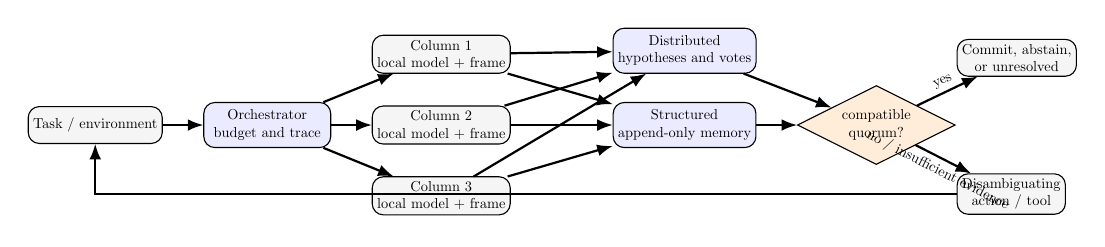
\begin{tikzpicture}[scale=0.52, transform shape,
  node distance=7mm and 10mm,
  box/.style={draw, rounded corners, align=center, minimum height=9mm, minimum width=25mm, fill=gray!8},
  state/.style={draw, rounded corners, align=center, minimum height=11mm, minimum width=31mm, fill=blue!8},
  decision/.style={draw, diamond, aspect=2, align=center, fill=orange!15},
  link/.style={-{Latex[length=2mm]}, thick}
]
\node[box] (task) {Task / environment};
\node[state, right=of task] (orch) {Orchestrator\\budget and trace};
\node[box, above right=of orch] (c1) {Column 1\\local model + frame};
\node[box, right=of orch] (c2) {Column 2\\local model + frame};
\node[box, below right=of orch] (c3) {Column 3\\local model + frame};
\node[state, right=25mm of c2] (mem) {Structured\\append-only memory};
\node[state, above=of mem] (hyp) {Distributed\\hypotheses and votes};
\node[decision, right=of mem] (vote) {compatible\\quorum?};
\node[box, below right=of vote] (active) {Disambiguating\\action / tool};
\node[box, above right=of vote] (out) {Commit, abstain,\\or unresolved};
\draw[link] (task) -- (orch);
\draw[link] (orch) -- (c1);
\draw[link] (orch) -- (c2);
\draw[link] (orch) -- (c3);
\draw[link] (c1) -- (mem);
\draw[link] (c2) -- (mem);
\draw[link] (c3) -- (mem);
\draw[link] (c1) -- (hyp);
\draw[link] (c2) -- (hyp);
\draw[link] (c3) -- (hyp);
\draw[link] (hyp) -- (vote);
\draw[link] (mem) -- (vote);
\draw[link] (vote) -- node[above, sloped] {yes} (out);
\draw[link] (vote) -- node[below, sloped] {no / insufficient evidence} (active);
\draw[link] (active) -| (task);
\end{tikzpicture}
\caption{CCM architecture. The arrows represent explicit state and observation contracts; the diagram does not imply biological correspondence.}
\label{fig:ccm-architecture}
\end{figure}

\subsection{Reference frames as computation}

A CCM reference frame is not a persona, topic, namespace, domain, or agent perspective. It is a navigable state space
\[
  F=(f, k, o, s, T, O),
\]
where $f$ is a stable identity, $k$ is the frame kind, $o$ is the origin, $s$ is the current state, $T$ is a set of validated transitions, and $O$ maps locations to observation identifiers. A transition $(a,s_i,s_j)\in T$ is valid only when the current state is $s_i$; an observation is attachable only when its frame and location are valid.

The first concrete example is spatial/object-like. A sensor observes a mug feature at object-local location \texttt{handle\_left}; action \texttt{rotate\_90} moves the state to \texttt{handle\_top}; the frame predicts an observation at that location. The second is conceptual. A claim begins at \texttt{claim\_unresolved}; action \texttt{inspect\_source\_a} moves to \texttt{claim\_supported} when the source observation supports the claim; a competing claim remains open if the observation does not discriminate. Both examples contain a state, a transition, a predicted next location, and evidence associated with a location.

\subsection{Columns}

A column is a local model plus a bounded state owner. It is not merely one agent or one prompt. Its minimum state contains local observation identifiers, a reference-frame state, one or more candidate hypotheses, evidence identifiers, confidence, uncertainty, provenance, requested next action, and received peer states. Columns may share a base model or use heterogeneous models; v0.1.0 exposes specialization labels but does not claim a trained specialization.

The standard interface is:

\begin{verbatim}
observe(observation)
update_hypotheses(candidates)
propose_action(available_actions)
emit_state()
receive_peer_state(peer_state)
vote()
commit(status)
\end{verbatim}

The interface separates local update from communication. A peer receives a serializable state, not hidden reasoning. A column can be committed, abstained, or unresolved by the orchestrator.

\subsection{CCM memory model}

CCM memory is neither conversation history, a scratchpad, ordinary RAG, a vector index, nor an assertion that episodic, semantic, and procedural memory have been biologically reconstructed. It is a structured, append-only observation ledger. The v0.1.0 object schema is:

\begin{longtable}{@{}p{0.22\linewidth}p{0.69\linewidth}@{}}
\toprule
Field & Contract \\
\midrule
object\_id & Stable unique identity; duplicate writes are rejected. \\
content & Human-readable observation payload. \\
frame\_id, location & Reference-frame identity and state/location. \\
source, provenance & Origin and trace link; required for every object. \\
sequence, timestamp & Ordered run-local history; timestamps are stored at run level. \\
confidence, validation\_state & Explicit quality and external validation status. \\
relations & Structured relations such as support or contradiction. \\
embedding & Optional future field; not used by the v0.1.0 symbolic adapter. \\
\bottomrule
\end{longtable}

Historical observations cannot be silently mutated. A model-generated hypothesis is not accepted as an external observation. Conflicting observations remain separate records and are visible to consensus and the run trace.

\subsection{Structured voting}

A vote is a tuple containing \texttt{vote\_id}, \texttt{column\_id}, \texttt{hypothesis\_id}, \texttt{hypothesis}, and confidence. A hypothesis contains a claim, frame, location, evidence identifiers, provenance, confidence, uncertainty, and optional requested action. Two hypotheses are compatible only when their normalized claim, frame identity, and location agree. Structured consensus sums confidence within compatible groups, requires a minimum quorum and confidence, and requires a margin over the runner-up. Ties and low-confidence groups are not forced into an answer. This differs from majority voting, self-consistency, debate, confidence-weighted answer aggregation, and judge-model aggregation because the primary unit is a frame-associated hypothesis with explicit evidence.

\subsection{Active evidence}

The active loop maintains competing hypotheses, identifies missing support, scores available actions by expected information gain divided by cost, executes one valid action, appends the resulting observation, and redistributes state. An action is not an answer and cannot create evidence without an environment response. If the action budget is exhausted, the system terminates with the best permitted non-commit outcome. The harness records action selection, returned observation, cost, and whether required evidence was retrieved.

\subsection{Primary algorithm}

Algorithm~\ref{alg:ccm} is implementation-independent pseudocode. It makes termination and disagreement explicit.

\begin{enumerate}
  \item Initialize $N$ columns, their reference frames, an empty append-only memory, and a run manifest.
  \item Observe the task/environment and write only externally returned observations with source and provenance.
  \item Each column updates local hypotheses and emits a structured state.
  \item Exchange states and group compatible hypotheses by frame, location, and claim.
  \item If a group satisfies quorum, confidence, and margin criteria, commit it.
  \item Otherwise, if uncertainty remains and an action budget is available, choose the highest information-gain-per-cost action.
  \item Execute the action, validate its returned observation, append it, and repeat from step 3.
  \item If evidence is insufficient, confidence is below threshold, or the budget is exhausted, abstain or terminate unresolved.
\end{enumerate}

\begin{table}[t]
\centering
\caption{CCM termination outcomes.}
\label{alg:ccm}
\begin{tabular}{ll}
\toprule
Outcome & Condition \\
\midrule
Committed & Compatible structured quorum, confidence, and margin are met. \\
Abstained & No safe commitment; aggregate confidence is below threshold. \\
Unresolved & Competing hypotheses remain too close or lack quorum. \\
\bottomrule
\end{tabular}
\end{table}

\subsection{Invariants}

The implementation and tests enforce the following invariants where feasible: every memory object has provenance; every hypothesis has a reference frame; every vote references an existing hypothesis; historical observations cannot be overwritten; disagreement is retained with its resolution mechanism; model-generated information cannot be represented as externally observed evidence; and each run has a deterministic configuration identity plus model, task, hardware, seed, and git metadata.

\section{TPAA integration context}

The original manuscript placed CCM ``under TPAA.'' In this release TPAA is retained as an integration context rather than placed in the title or treated as prerequisite knowledge. CCM can be evaluated as a module inside a broader multi-agent architecture with an orchestrator, tool boundary, event transport, and deployment policy. The paper's contribution remains understandable without TPAA: the testable unit is the CCM memory, reference-frame, column, active-evidence, and consensus protocol.

The integration boundary is intentionally narrow. An orchestrator supplies a task, model adapter, available actions, budgets, and trace sink. A column consumes observations and peer states and emits structured state. A tool returns an observation or an explicit failure. The transport may be local function calls or a future RPC/event layer; the v0.1.0 implementation uses local calls and has no cross-service deployment claim. This keeps the validation harness focused on architecture rather than vendor or topology lock-in.

\section{Preregistered evaluation protocol}

The authoritative registration is in \texttt{preregistration/}. The full configuration is the v0.1.0 file under \texttt{registered-configs/}; the smoke configuration is separate and is not a substitute for the campaign. The primary comparison is memory quality under matched task, history, model, and resource conditions.

\subsection{Primary memory baselines}

\scriptsize
\begin{longtable}{@{}p{0.16\linewidth}p{0.74\linewidth}@{}}
\toprule
ID & Definition \\
\midrule
M0 & No persistent memory; current task context only. \\
M1 & Full-history memory. \\
M2 & Periodically summarized textual memory. \\
M3 & Vector-similarity retrieval over historical observations. \\
M4 & Structured key/value or episodic memory. \\
M5 & Knowledge-graph memory where practical. \\
M6 & Full CCM: bounded local models, frames, history, recall, reconciliation, and optional active evidence. \\
M7 & CCM plus an optional ontology substrate; exploratory if implemented. \\
\bottomrule
\end{longtable}
\normalsize

The deterministic v0.1.0 adapter implements transparent symbolic controls for M0--M6. It does not claim to be a learned summarizer, embedding model, or production knowledge graph. The full registered campaign should use explicit model/runtime implementations where resources permit.

\subsection{CCM ablations}

\begin{longtable}{@{}p{0.25\linewidth}p{0.65\linewidth}@{}}
\toprule
Ablation & Removed or changed mechanism \\
\midrule
\texttt{CCM-NoRF} & Explicit reference-frame constraints. \\
\texttt{CCM-NoModules} & Multiple bounded columns; one local module remains. \\
\texttt{CCM-NoTemporal} & Temporal recall and current-state constraints. \\
\texttt{CCM-NoReconciliation} & Reconciliation-driven structured commit. \\
\texttt{CCM-NoActive} & Active evidence acquisition. \\
\texttt{CCM-FlatLedger} & Frame-aware organization; flat structured-ledger comparison. \\
\bottomrule
\end{longtable}

\subsection{Memory task classes}

The deterministic suite prioritizes persistent factual recall, temporal state, relational recall, conflicting evidence, state replacement/supersession, provenance recall, cross-frame integration, distractor resistance, long-horizon continuity, active evidence, incomplete information, and pure reasoning control. Each task has a stable ID, hidden answer, candidate hypotheses, explicit observations or actions, and required evidence where applicable.

\subsection{Metrics}

Primary metrics are recall precision, recall recall, state reconstruction accuracy, temporal accuracy, relation accuracy, provenance accuracy, contradiction preservation, false-memory rate, stale-state rate, and relevant-context density. Secondary metrics include downstream task success, unsupported-memory rate, context tokens, retrieval/update latency, storage bytes, relation count, index size, candidates examined, communication, calibration, abstention, unresolved outcomes, and failure taxonomy. Smoke tables expose these fields but do not constitute campaign results.

\subsection{Model scale and composition}

Model scale is a secondary dimension. Where practical, the same memory architecture should be evaluated across small local, larger open, and hosted/frontier model classes, measuring relative improvement from each model's baseline memory condition rather than asking whether a small model catches a frontier model. Multi-agent composition is exploratory: independent CCM-equipped agents may exchange bounded memory-derived state without requiring a shared global store.

\subsection{Resource accounting}

The harness records model invocations, input/output tokens, wall-clock latency, communication, bytes stored, object and relation counts, index size, recall candidates examined, context tokens produced, retrieval latency, update cost, and unavailable hardware/energy/API fields. Pareto analysis therefore compares memory quality against storage, retrieval latency, context, and compute.

\subsection{Statistical decision rules}

The unit of analysis is a task instance, paired by task ID and seed. The registered configuration uses three independent seeds and ten instances per task class. The analysis reports raw differences, 95\% percentile bootstrap confidence intervals using 10,000 resamples, paired effect sizes, and Holm correction across confirmatory comparisons. A minimum practically meaningful difference is 0.05 on the relevant bounded metric. Failures and timeouts remain in denominators; there is no silent outlier removal or outcome-dependent stopping.

\subsection{Negative results and provenance}

All registered instances, unresolved states, contradictions, abstentions, timeouts, and unavailable resource measurements remain in the analysis. Run manifests record configuration hash, Git commit, model/task versions, seed, hardware, timestamp, and raw output. Private chain-of-thought is neither required nor stored. The protocol makes no claim until the full campaign replaces the smoke status with traceable results.

\section{Reference implementation}

The repository is a standard-library-only Python reference implementation. The conceptual boundaries are explicit even where the v0.1.0 directory layout remains compact:

\begin{description}
  \item[\texttt{ccm/schemas}.] Stable contracts for observations, relations, state, hypotheses, transitions, predictions, votes, actions, and column state.
  \item[\texttt{ccm/memory}.] Append-only observation history, temporal queries, supersession, and provenance-bearing write/retrieve operations.
  \item[\texttt{ccm/recall}.] Bounded lexical recall, current-state selection, conflict visibility, and context assembly.
  \item[\texttt{ccm/reference\_frames}.] Valid state transitions and frame/location constraints.
  \item[\texttt{ccm/column}.] Bounded local modeling-unit interface. A column is not an agent.
  \item[\texttt{ccm/consensus}.] Reconciliation outcomes and optional structured quorum voting.
  \item[\texttt{ccm/active\_evidence}.] Information-gain-per-cost action selection.
  \item[\texttt{ccm/adapters}.] Provider-neutral model adapter contract, including an injected JSON-boundary LLM adapter with no network dependency.
  \item[\texttt{ccm/orchestration}.] Local execution loop that records recall, context assembly, reconciliation, optional action, and explicit termination.
  \item[\texttt{experiments} and \texttt{evaluation}.] Deterministic task worlds, M0--M6 controls, CCM ablations, manifests, memory metrics, resource accounting, and statistical utilities.
\end{description}

The symbolic \texttt{ToyModel} is intentionally deterministic and inspectable. It supports unit, invariant, integration, and smoke validation; it is not described as a language-model result. An actual model can implement the injected adapter interface while preserving the observation/provenance boundary.

\subsection{Testing surface}

Tests cover immutable observations, duplicate handling, required provenance, hypothesis/observation separation, historical and current queries, supersession, late temporal validity, valid and invalid reference-frame transitions, and column isolation. They also cover agreement, complementary evidence, contradiction, unknown and unresolved outcomes, bounded recall, distractor rejection, multi-hop state, provenance return, bounded context assembly, deterministic task generation, manifests, and generated smoke record shape.

\subsection{Reproducibility}

Every run emits JSONL records and a manifest with configuration hash, protocol version, model and task version, seed, hardware metadata, Git commit, timestamps, resource fields, structured trace, and output path. The repository contains no hosted credentials and the smoke path has no network dependency.

\section{Results status}

The full registered campaign has not been executed. This release therefore does not report a scientific estimate for H1--H10 and does not claim that CCM improves memory quality. The checked-in smoke artifacts are deterministic software-validation outputs used to verify task generation, schema contracts, trace completeness, resource fields, analysis, and paper-table generation.

The generated table in Table~\ref{tab:smoke-memory} is intentionally labelled smoke validation. It exposes memory-oriented fields such as recall, temporal accuracy, provenance, and context tokens; it must not be interpreted as a comparison of language-model capability. A future registered run will replace protocol-state language only after all configured seeds, task instances, baselines, ablations, matched resource views, confidence intervals, effect sizes, and failure analyses are present.

\begin{table}[t]
\centering
\caption{Deterministic smoke-validation schema. Values are generated from the checked-in symbolic adapter and are not scientific campaign results.}
\label{tab:smoke-memory}
% Generated by evaluation.reporting.analyze; do not edit manually.
\begin{tabular}{lrrr}
\toprule
Strategy & Success rate & False consensus & Model calls \\
\midrule
B0 & 0.556 & 0.444 & 1.0 \\
B1 & 0.667 & 0.333 & 1.0 \\
B2 & 0.667 & 0.333 & 5.0 \\
B3 & 0.556 & 0.444 & 3.0 \\
B4 & 0.556 & 0.444 & 3.0 \\
B5 & 0.556 & 0.444 & 3.0 \\
CCM-Full & 0.778 & 0.000 & 4.3 \\
CCM-NoActive & 0.556 & 0.286 & 3.0 \\
CCM-NoVote & 0.889 & 0.111 & 4.3 \\
\bottomrule
\end{tabular}

\end{table}

\section{Discussion}

Some failures attributed to agent reasoning may arise because the model is repeatedly asked to reconstruct world state from incomplete, noisy, semantically retrieved, or compressed history. CCM proposes a different systems boundary: preserve historical observations and provenance, derive current state explicitly, organize local models relative to frames, and return bounded context through a recall interface.

The design has several intended advantages. Temporal semantics separate what was true from what is true now. Provenance makes a recalled claim auditable. Modular local models may reduce irrelevant-memory contamination and permit complementary state rather than a single collapsed summary. Reconciliation can preserve contradictions and unknown outcomes. Active evidence can make a missing observation an explicit next step rather than an unsupported completion.

These advantages have costs. Structured state requires schemas, update policies, conflict handling, indexing, and additional storage. Multiple columns can correlate errors when they share one model. Recall and context assembly introduce latency and implementation complexity. A structured representation can also encode the wrong ontology or miss information that a free-form transcript retained. The protocol therefore measures memory quality jointly with storage, latency, context, and compute.

The model-scale interaction is deliberately secondary. A stronger model may benefit from the same structured memory, and a weaker model may benefit more or less depending on its ability to use the context. The relevant comparison is relative improvement from each model's matched memory baseline, not a promise that small models catch frontier models. Multi-agent composition is similarly a follow-on question: independent CCM instances may exchange bounded state, but CCM does not define the outer topology.

Ontology integration is optional. An ontology can constrain valid entities and predicates, while CCM retains observed instances and their time-dependent state. A future ontology-backed experiment should be treated as a distinct extension rather than folded into the core definition. Likewise, the ``world model'' label is limited here to explicit transition and prediction contracts; the symbolic harness does not establish a learned world model.

Finally, the Thousand Brains analogy is a design inspiration with a strict boundary. If TBT is incomplete or revised, CCM should still stand or fall on its own memory contracts, tests, and empirical evidence.

\section{Related work and threats to validity}

\subsection{Novelty matrix}

The matrix is a conservative design comparison, not a claim that every system in a category has identical capabilities. ``Varies'' indicates that the property depends on the implementation.

\scriptsize
\setlength{\tabcolsep}{2pt}
\begin{longtable}{@{}p{0.14\linewidth}p{0.07\linewidth}p{0.07\linewidth}p{0.07\linewidth}p{0.07\linewidth}p{0.07\linewidth}p{0.07\linewidth}p{0.09\linewidth}p{0.09\linewidth}@{}}
\toprule
Approach & Hist. & Rel. & Time & Frame & Prov. & Local & Conflict & Active \\
\midrule
Transcript & yes & var. & impl. & no & text & no & var. & no \\
Summary & comp. & var. & lossy & no & lossy & no & lossy & no \\
Vector memory & yes & no & var. & no & var. & no & var. & no \\
KG memory & yes & yes & var. & no & var. & no & var. & no \\
Episodic memory & yes & var. & var. & var. & var. & var. & var. & var. \\
TBP/Monty & yes & yes & var. & loc. & var. & mod. & var. & yes \\
CCM & yes & yes & exp. & exp. & req. & bound. & kept & opt. \\
\bottomrule
\end{longtable}
\normalsize
\setlength{\tabcolsep}{6pt}

CCM's distinguishing engineering claim is the combination of immutable provenance-bearing observations, explicit temporal/current-state separation, reference-frame constraints, bounded local models, recall/context assembly, and reconciliation that preserves contradiction. The paper does not claim that CCM invented persistent memory, graphs, reference frames, active information acquisition, or multiple agents.

\subsection{Threats to validity}

\begin{description}
  \item[Biological analogy.] TBT, TBP/Monty, HTM, SDRs, and CCM are distinct. The paper makes no neural or cortical equivalence claim.
  \item[Toy adapter.] The symbolic adapter validates software contracts, not natural-language capability. Full claims require model-backed runs with exact model/runtime provenance.
  \item[Task validity.] Synthetic tasks may not represent real agent workloads. The protocol therefore labels them as controlled validation and requires future domain tasks before broad generalization.
  \item[Metric validity.] Recall precision, temporal accuracy, provenance, and context density are operational measures, not complete measures of useful memory. Downstream task success remains secondary but necessary.
  \item[Correlated columns.] Shared-model columns are not independent evidence. The manifest records model identity and the protocol includes a no-modules condition.
  \item[Retriever bias.] Lexical smoke recall is not a vector retriever. M3 must use a real embedding/retrieval implementation in a registered empirical run.
  \item[Resource measurement.] Local runs may not expose energy, accelerator time, or API cost. Those fields remain unavailable rather than imputed.
  \item[Negative outcomes.] Contradictions, abstentions, unresolved results, failures, and missing resources remain in denominators. No outcome-dependent stopping or silent removal is permitted.
\end{description}

\subsection{Scope and reproducibility}

All public claims must be classified as primary literature fact, project implementation fact, interpretation, CCM design choice, or hypothesis. The source bibliography uses primary TBT papers, project sources, memory/retrieval work, and carefully bounded secondary comparisons. The checked-in code, protocol, manifests, tests, and paper build provide the reproducibility surface.

\section{Conclusion}

CCM is presented here as a concrete, inspectable distributed-agent architecture rather than a reconstruction of cortical computation. It translates selected Thousand Brains-inspired ideas into explicit reference frames, columns, structured memory, active evidence, and consensus contracts. The repository exposes those mechanisms, registers hypotheses and ablations, controls test-time resources, records provenance, and preserves negative outcomes as valid research results.

The v0.1.0 contribution is methodological transparency: a reader can inspect and run the architecture before the full empirical campaign is collected. Whether CCM recovers useful capability under constrained budgets, and where it fails to compensate for model scale, remains an empirical question for the registered evaluation and future release.

\appendix
\section{Preregistration summary}

This appendix summarizes the frozen protocol. The YAML and JSON files in \texttt{preregistration/} are authoritative for execution.

\subsection{Hypotheses}

\begin{longtable}{p{0.09\linewidth}p{0.78\linewidth}}
\toprule
ID & Registered statement \\
\midrule
H1 & CCM-Full improves task success over B0 on the full task suite. \\
H2 & CCM-Full improves task success over B3 under comparable call and token budgets. \\
H3 & Removing explicit reference frames reduces performance on persistent state transformation tasks. \\
H4 & Removing active evidence reduces performance on disambiguation tasks. \\
H5 & Structured consensus reduces false consensus relative to answer-level majority voting. \\
H6 & CCM benefit varies by task class, with smaller gains on pure reasoning controls than on memory/evidence tasks. \\
\bottomrule
\end{longtable}

\subsection{Analysis commitments}

Three independent seeds and ten instances per task class are registered. Task success is binary and bounded; abstention and unresolved outcomes are failures for this metric. Confidence calibration, abstention quality, false consensus, memory precision/recall, evidence utilization, convergence steps, communication overhead, failure categories, and resources are secondary outcomes. Report raw effects, 95\% bootstrap confidence intervals, effect sizes, and practical significance; apply Holm correction across primary pairwise tests; retain timeouts and failures; perform no outlier removal or outcome-dependent stopping.

\subsection{Negative-results and version policy}

The registered results will be published whether the hypotheses are supported, qualified, or rejected. A component that contributes nothing will be reported. Corrections that do not alter registered elements may be v0.2.x releases with changelog entries. Changes to hypotheses, metrics, baselines, exclusions, or thresholds require a deviation record and a new protocol version. v1.0.0 requires all registered seeds, raw and processed data, generated tables and figures, matched-budget analyses, ablations, failure taxonomy, resource Pareto analysis, and evidence-based abstract/conclusion updates.


% refs.bib is the editable bibliography source. refs.bbl is checked in so the
% bundled Tectonic path can reproduce the PDF without an external BibTeX binary.
\input{refs.bbl}
\end{document}
